\documentclass[10pt,a4paper]{article}
\usepackage[T1]{fontenc}
\usepackage{lmodern}
\usepackage[margin=19mm,headheight=13pt,headsep=5mm,footskip=9mm]{geometry}
\usepackage{amsmath,amssymb,bm,graphicx,booktabs,array,longtable}
\usepackage[font=small,labelfont=bf]{caption}
\captionsetup{hypcap=false}
\usepackage{xcolor,fancyhdr}
\usepackage[hidelinks]{hyperref}
\usepackage{microtype}
\definecolor{ink}{RGB}{27,46,65}
\pagestyle{fancy}\fancyhf{}
\fancyhead[L]{\small\textcolor{ink}{Membrane stability and flow-driven buckling}}
\fancyhead[R]{\small Integrated report | October 2026}
\fancyfoot[C]{\small\thepage}
\renewcommand{\headrulewidth}{0.3pt}
\setlength{\parskip}{4pt}\setlength{\parindent}{0pt}
\setlength{\emergencystretch}{2em}
\newcommand{\SL}{\mathrm{SL}}
\newcommand{\dd}{\mathrm{d}}
\newcommand{\e}{\mathrm{e}}
\newcommand{\Real}{\operatorname{Re}}
\newcommand{\Imag}{\operatorname{Im}}
\newcommand{\tr}{\operatorname{tr}}
\newcommand{\fig}[4]{\par\medskip\noindent\begin{minipage}{\linewidth}\centering\reportgraphic{#1}{#4}\captionof{figure}[Research figure]{#2}\label{#3}\end{minipage}\par\medskip}
\raggedbottom
\makeatletter
\renewcommand*\l@section{\@dottedtocline{1}{0em}{2.5em}}
\renewcommand*\l@subsection{\@dottedtocline{2}{2.5em}{3.2em}}
\makeatother

\newcommand{\source}[1]{\path{#1}}
\hypersetup{pdftitle={Flow-driven buckling and mechanochemical instabilities of membranes with protein inclusions},pdfauthor={Copy Stage research project}}

% Individual figure sizing and lossless panel layouts. All original image bytes
% are retained; trim/clip only changes the displayed viewport in this document.
\newcommand{\reportgraphic}[2]{%
  \ifcsname reportlayout@#1\endcsname
    \csname reportlayout@#1\endcsname
  \else
    \includegraphics[width=\linewidth,height=#2,keepaspectratio]{#1}%
  \fi}
% Trim amounts are fractions of the original image width/height.
\newdimen\reportLeft
\newdimen\reportBottom
\newdimen\reportRight
\newdimen\reportTop
\newcommand{\reportpanel}[7]{%
  \begingroup
  \setbox0=\hbox{\includegraphics{#1}}%
  \reportLeft=#3\wd0\relax
  \reportBottom=#4\ht0\relax
  \reportRight=#5\wd0\relax
  \reportTop=#6\ht0\relax
  \edef\reportinclude{\noexpand\includegraphics[width=#2,height=#7,keepaspectratio,
    trim={\the\reportLeft\space\the\reportBottom\space\the\reportRight\space\the\reportTop},clip]{#1}}%
  \reportinclude%
  \endgroup}
\expandafter\def\csname reportlayout@figures/wake_check_projector_equivalence.png\endcsname{%
  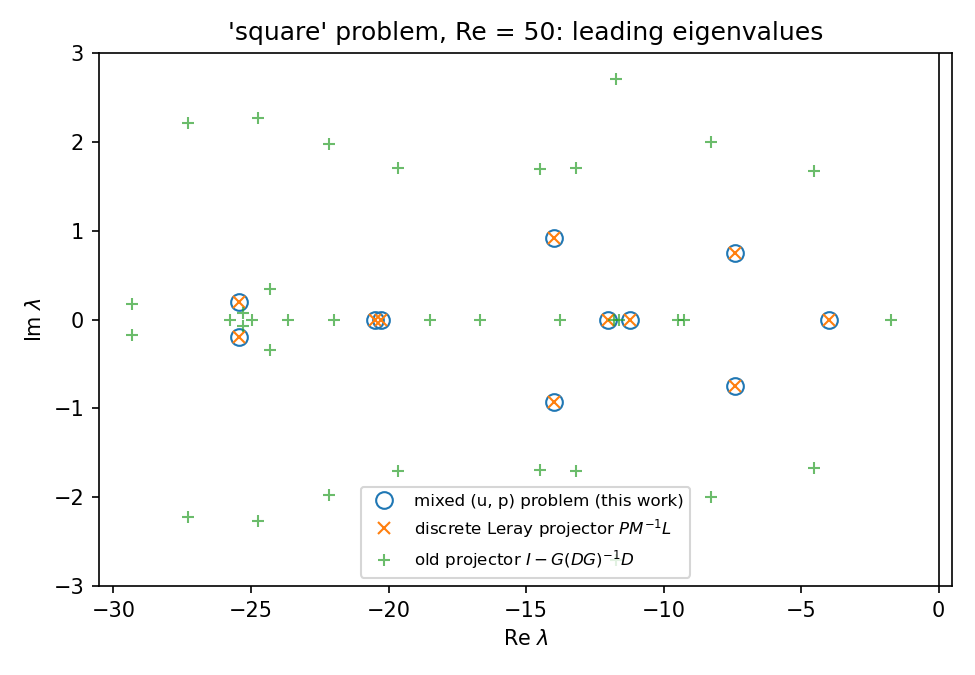
\includegraphics[width=0.76\linewidth,height=90mm,keepaspectratio]{figures/wake_check_projector_equivalence.png}%
}
\expandafter\def\csname reportlayout@figures/membrane_flat_ring_R5_coarse.png\endcsname{%
  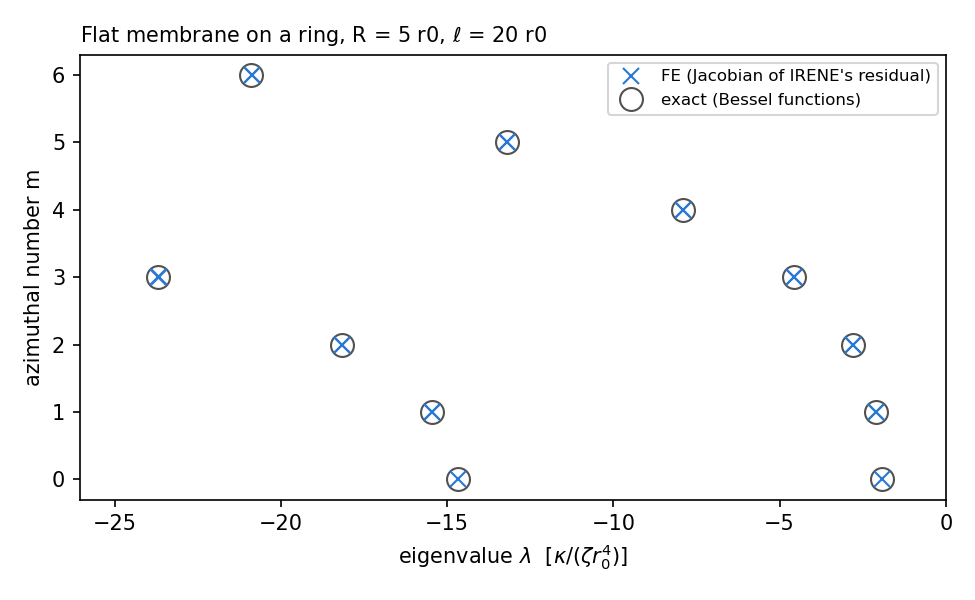
\includegraphics[width=0.70\linewidth,height=82mm,keepaspectratio]{figures/membrane_flat_ring_R5_coarse.png}%
}
\expandafter\def\csname reportlayout@figures/membrane_flat_ring_R5_fine.png\endcsname{%
  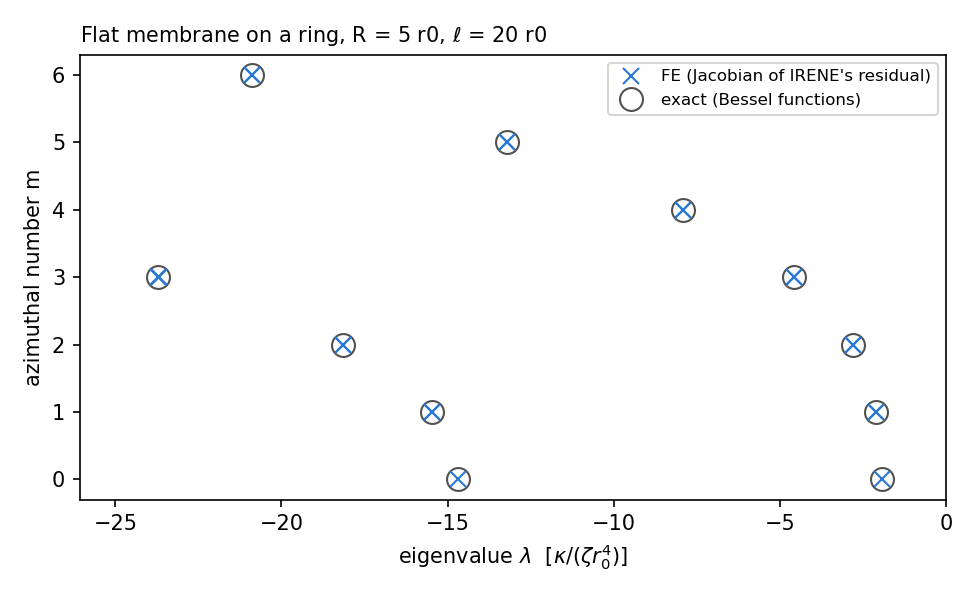
\includegraphics[width=0.70\linewidth,height=82mm,keepaspectratio]{figures/membrane_flat_ring_R5_fine.png}%
}
\expandafter\def\csname reportlayout@figures/wake_spectra.png\endcsname{%
  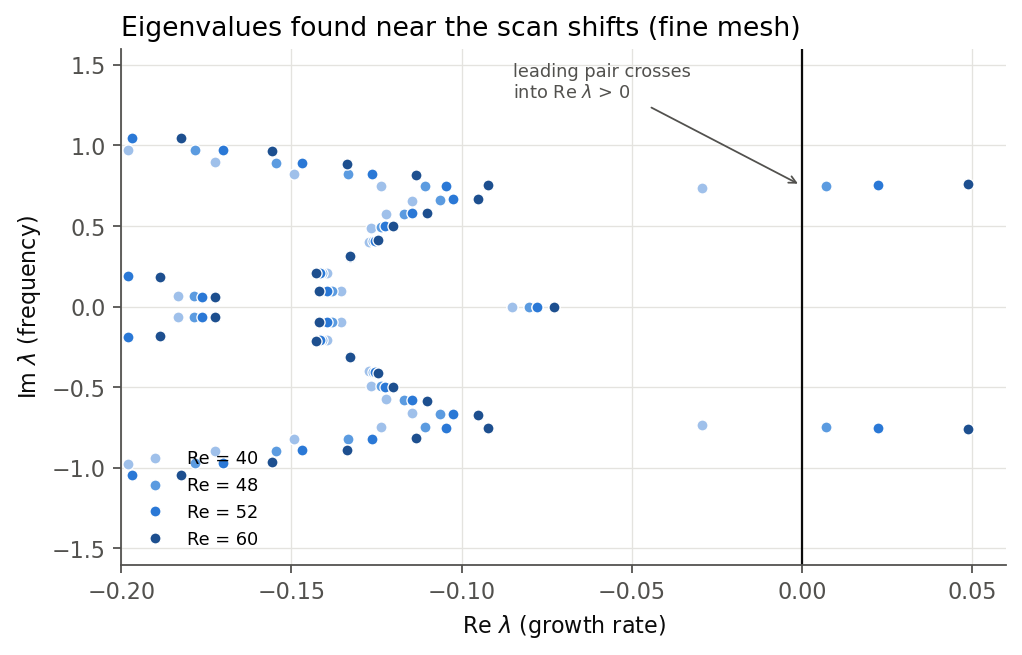
\includegraphics[width=0.78\linewidth,height=100mm,keepaspectratio]{figures/wake_spectra.png}%
}
\expandafter\def\csname reportlayout@figures/wake_eigenvalue_trajectories.png\endcsname{%
  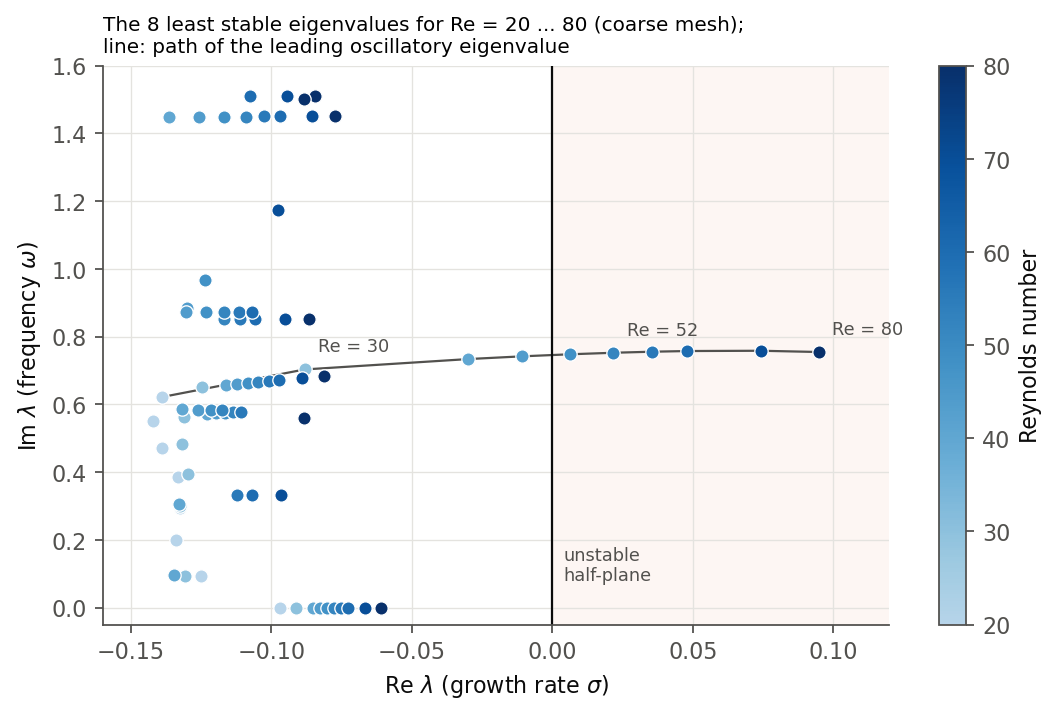
\includegraphics[width=0.78\linewidth,height=100mm,keepaspectratio]{figures/wake_eigenvalue_trajectories.png}%
}
\expandafter\def\csname reportlayout@figures/wake_dns_vorticity.png\endcsname{%
  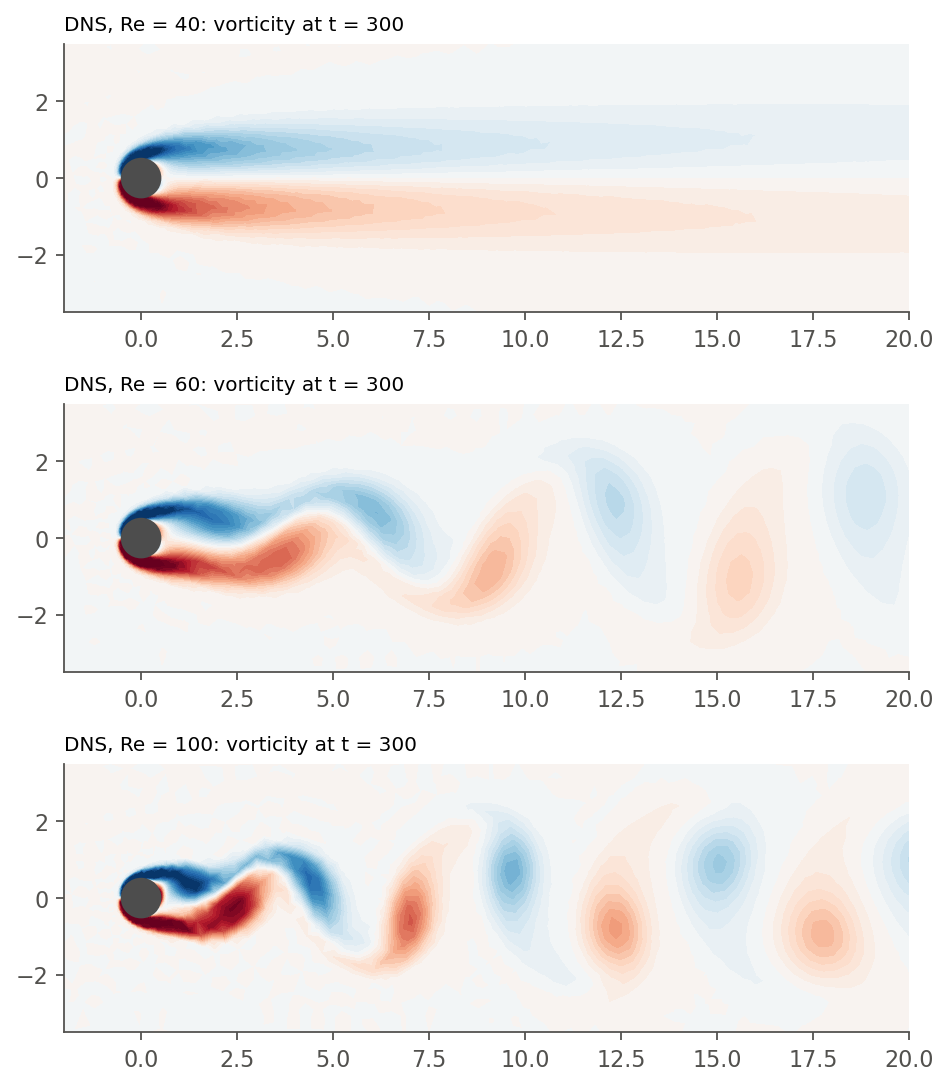
\includegraphics[width=0.64\linewidth,height=112mm,keepaspectratio]{figures/wake_dns_vorticity.png}%
}
\expandafter\def\csname reportlayout@figures/membrane_check_force_methods.png\endcsname{%
  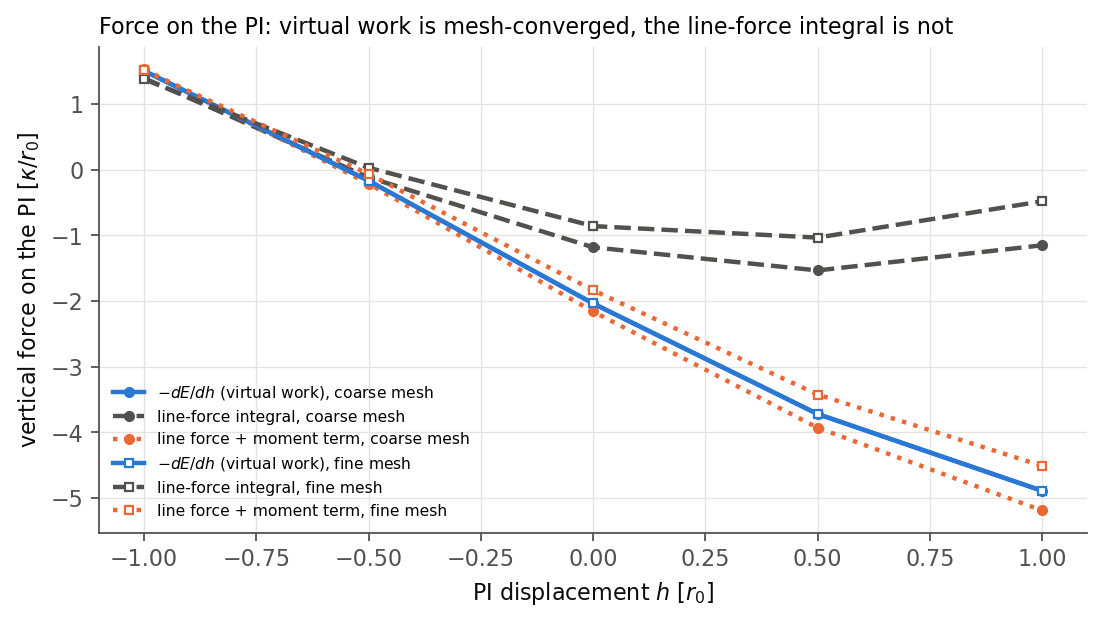
\includegraphics[width=0.82\linewidth,height=92mm,keepaspectratio]{figures/membrane_check_force_methods.png}%
}
\expandafter\def\csname reportlayout@figures/membrane_profiles_ring_R10_tan0.png\endcsname{%
  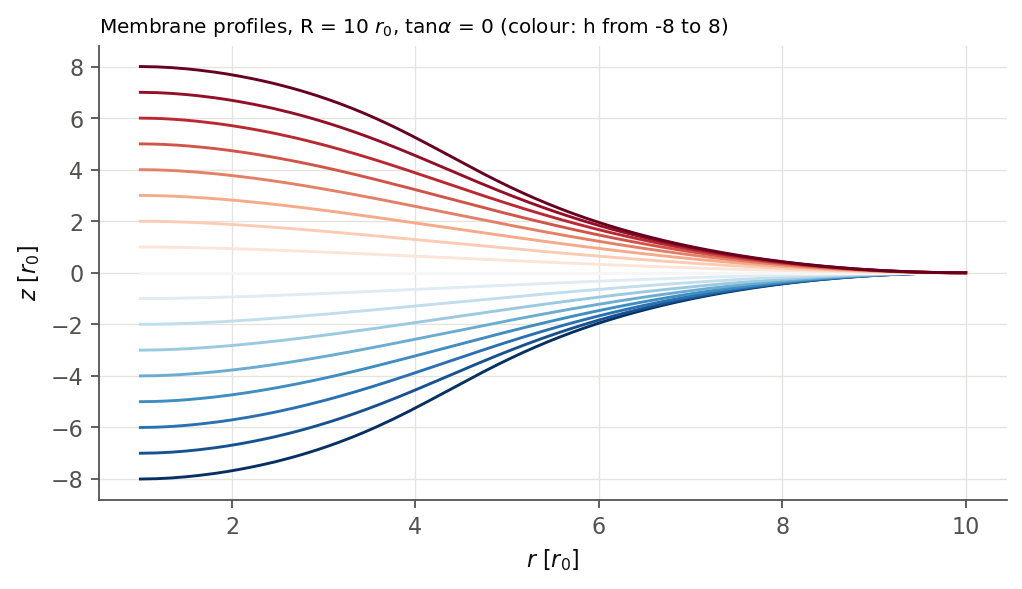
\includegraphics[width=0.76\linewidth,height=85mm,keepaspectratio]{figures/membrane_profiles_ring_R10_tan0.png}%
}
\expandafter\def\csname reportlayout@figures/membrane_profiles_ring_R10_tan0.5.png\endcsname{%
  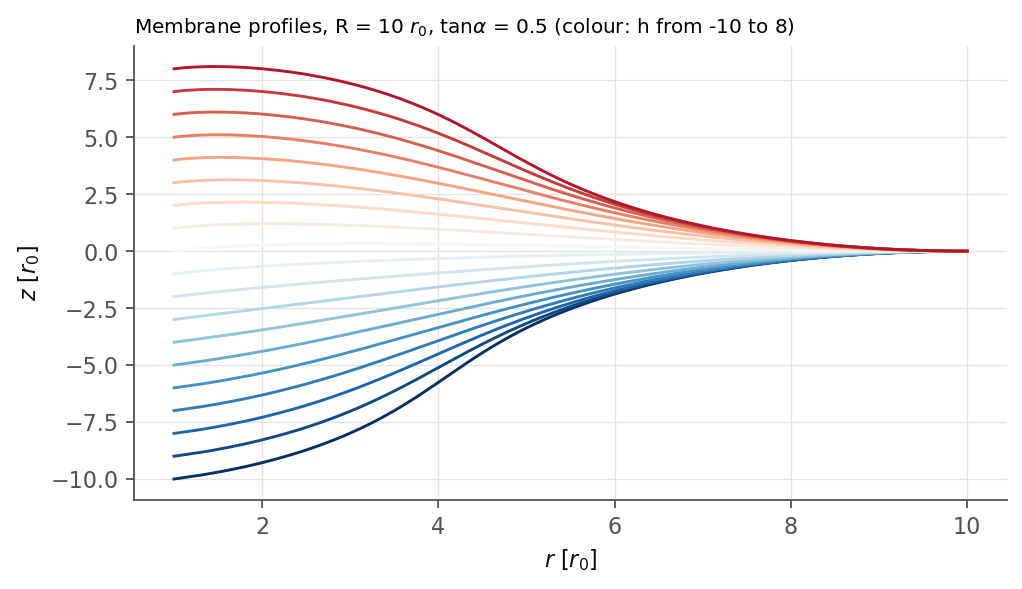
\includegraphics[width=0.76\linewidth,height=85mm,keepaspectratio]{figures/membrane_profiles_ring_R10_tan0.5.png}%
}
\expandafter\def\csname reportlayout@figures/membrane_profiles_ring_R10_tan1.png\endcsname{%
  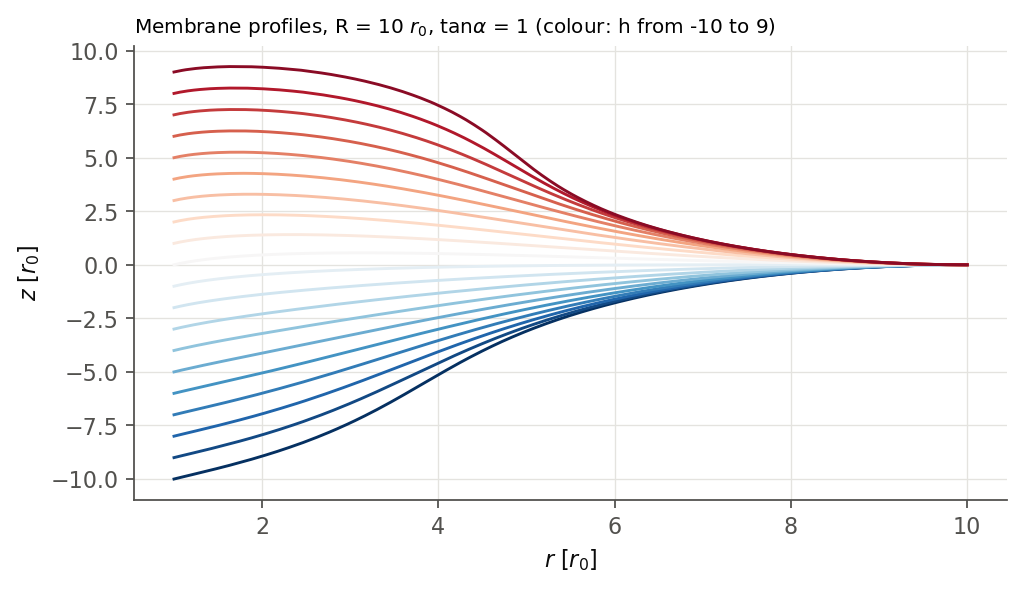
\includegraphics[width=0.76\linewidth,height=85mm,keepaspectratio]{figures/membrane_profiles_ring_R10_tan1.png}%
}
\expandafter\def\csname reportlayout@figures/membrane_profiles_ring_R5_tan0.5.png\endcsname{%
  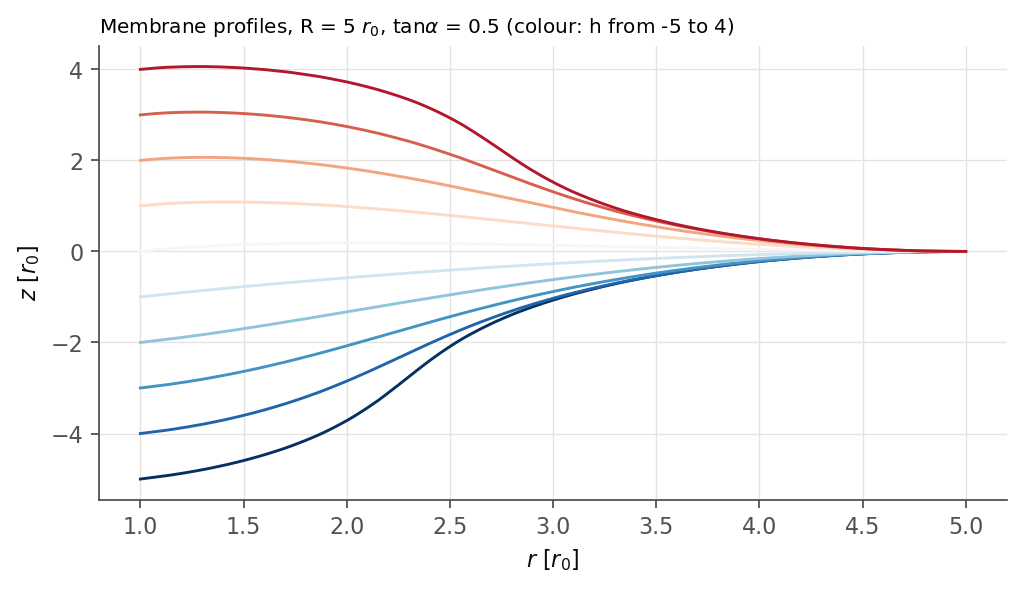
\includegraphics[width=0.76\linewidth,height=85mm,keepaspectratio]{figures/membrane_profiles_ring_R5_tan0.5.png}%
}
\expandafter\def\csname reportlayout@figures/membrane_profiles_ring_R30_tan0.5.png\endcsname{%
  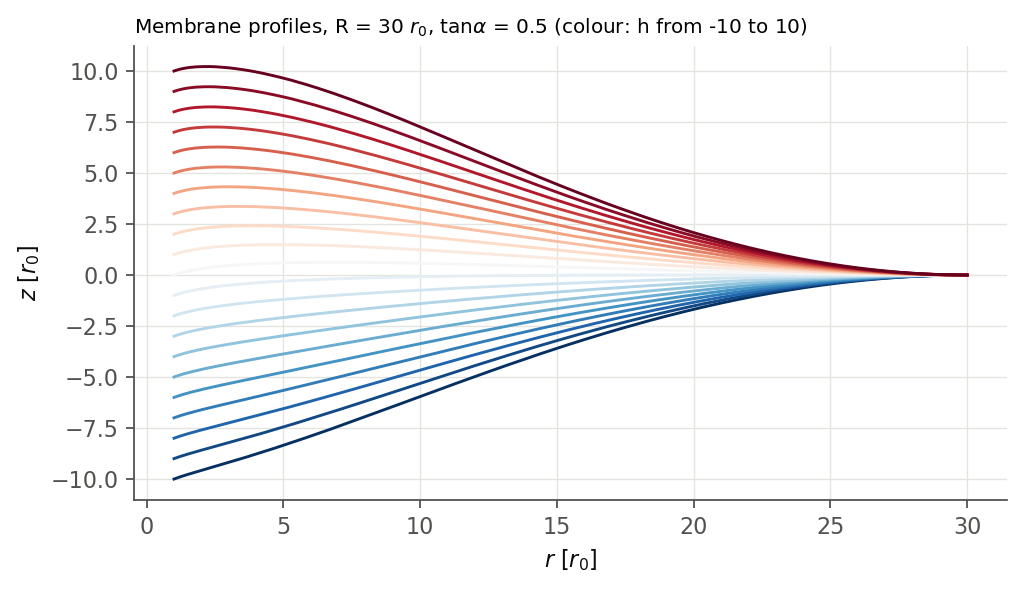
\includegraphics[width=0.76\linewidth,height=85mm,keepaspectratio]{figures/membrane_profiles_ring_R30_tan0.5.png}%
}
\expandafter\def\csname reportlayout@figures/membrane_ring_force_physical_units.png\endcsname{%
  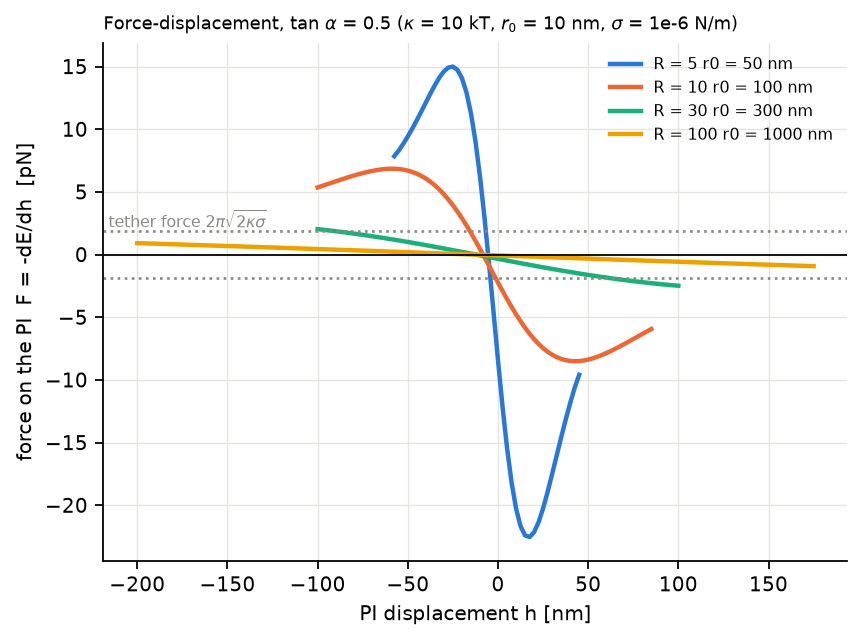
\includegraphics[width=0.72\linewidth,height=105mm,keepaspectratio]{figures/membrane_ring_force_physical_units.png}%
}
\expandafter\def\csname reportlayout@figures/membrane_flow_pre_SLc_vs_tension.png\endcsname{%
  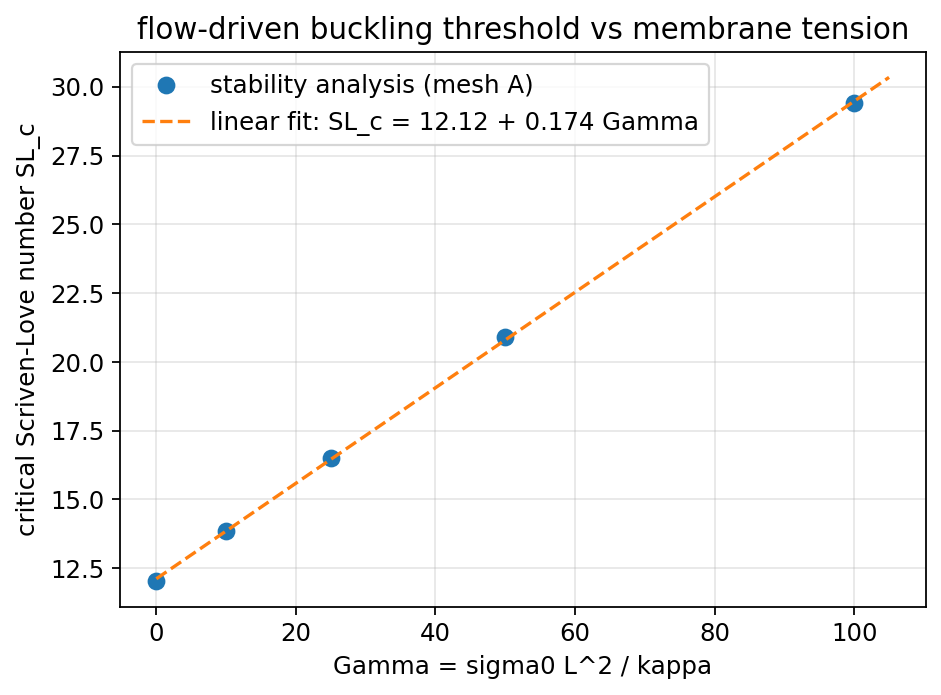
\includegraphics[width=0.70\linewidth,height=100mm,keepaspectratio]{figures/membrane_flow_pre_SLc_vs_tension.png}%
}
\expandafter\def\csname reportlayout@figures/membrane_flow_pre_tension_centreline.png\endcsname{%
  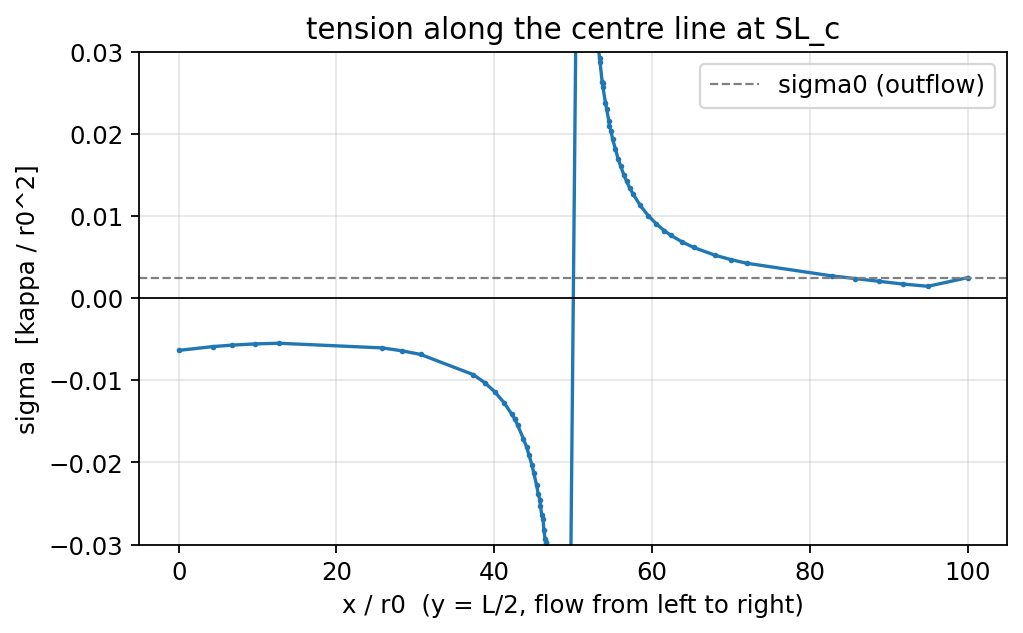
\includegraphics[width=0.66\linewidth,height=90mm,keepaspectratio]{figures/membrane_flow_pre_tension_centreline.png}%
}
\expandafter\def\csname reportlayout@figures/membrane_flow_time_check.png\endcsname{%
  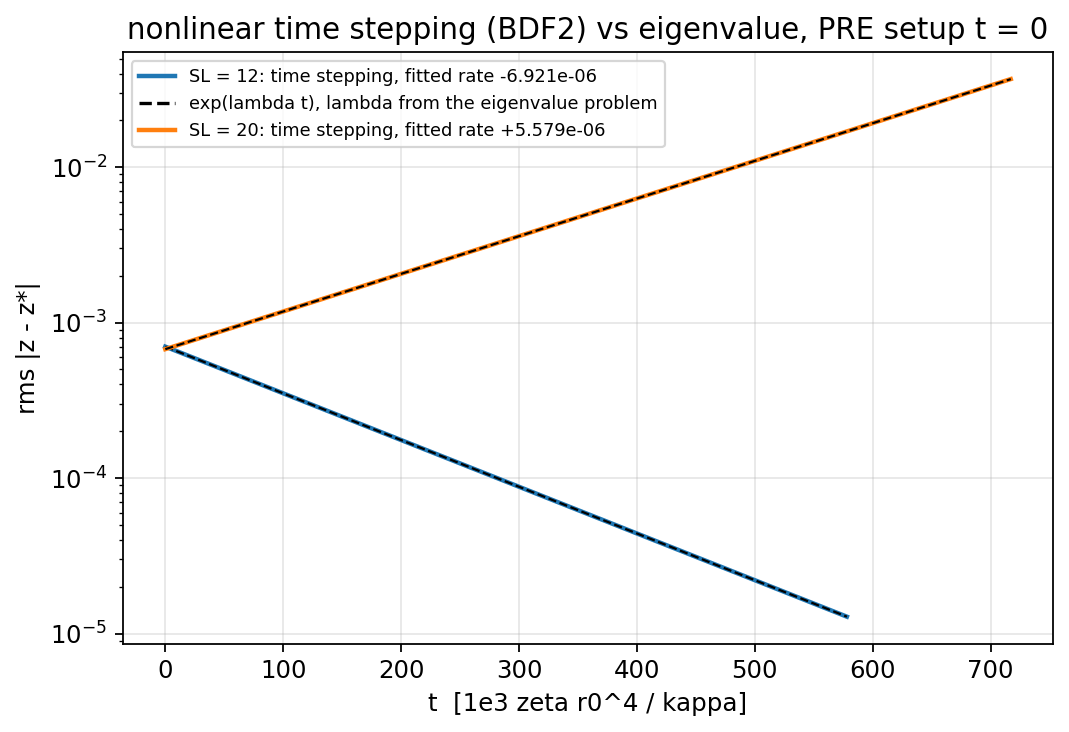
\includegraphics[width=0.76\linewidth,height=100mm,keepaspectratio]{figures/membrane_flow_time_check.png}%
}
\expandafter\def\csname reportlayout@figures/membrane_flow2_threshold_vs_tension.png\endcsname{%
  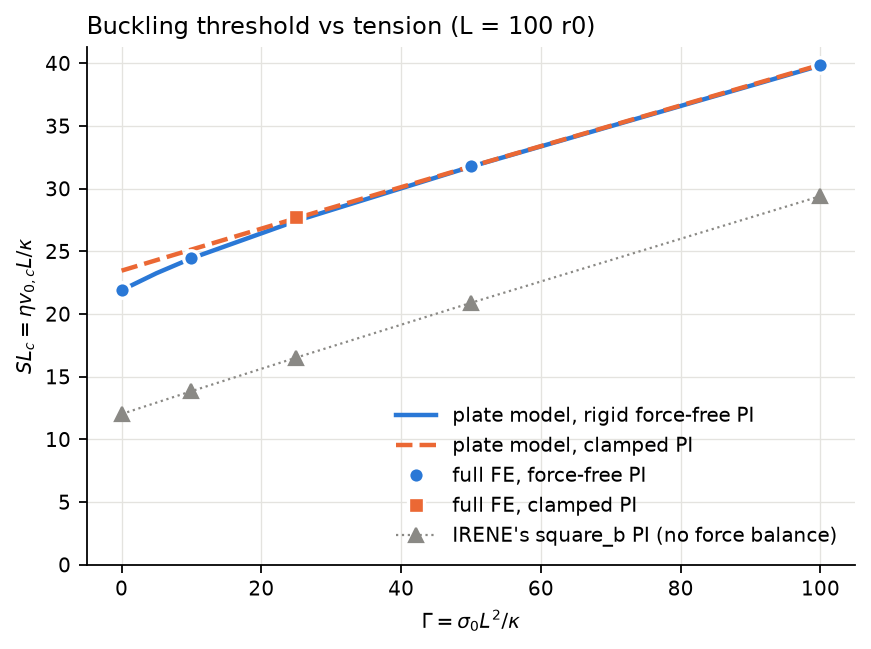
\includegraphics[width=0.70\linewidth,height=100mm,keepaspectratio]{figures/membrane_flow2_threshold_vs_tension.png}%
}
\expandafter\def\csname reportlayout@figures/membrane_flow2_friction.png\endcsname{%
  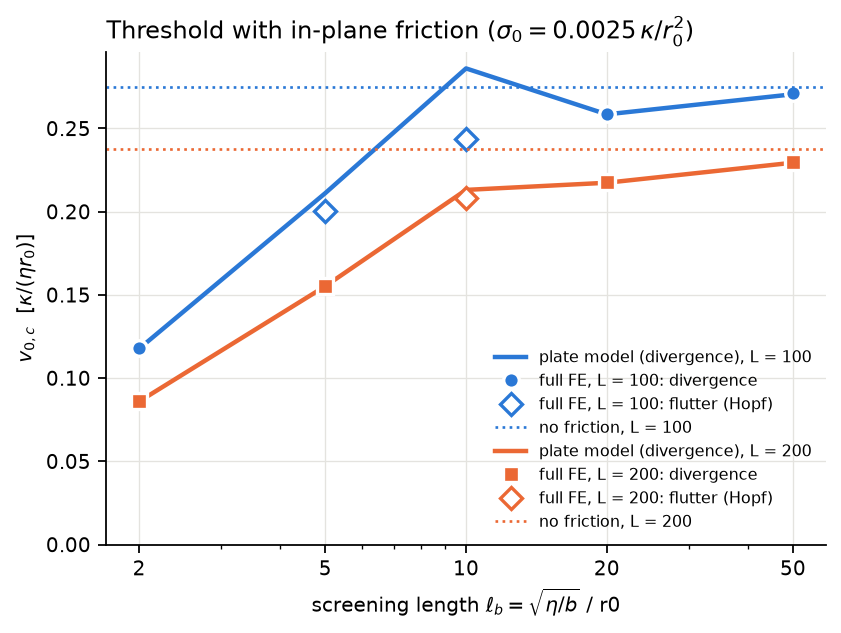
\includegraphics[width=0.72\linewidth,height=100mm,keepaspectratio]{figures/membrane_flow2_friction.png}%
}
\expandafter\def\csname reportlayout@figures/membrane_r6_wake.png\endcsname{%
  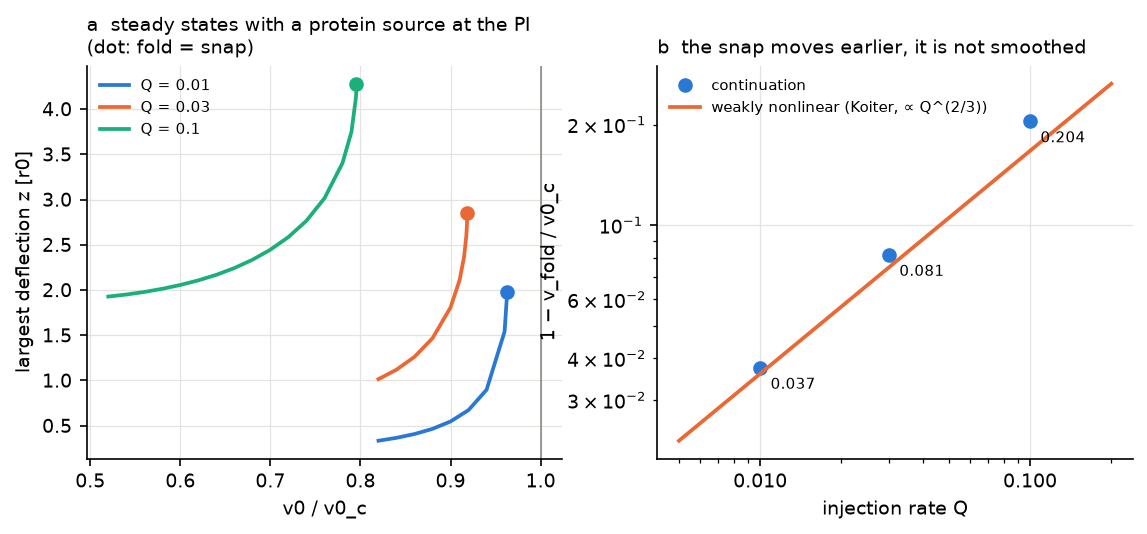
\includegraphics[width=0.86\linewidth,height=75mm,keepaspectratio]{figures/membrane_r6_wake.png}%
}
\expandafter\def\csname reportlayout@figures/membrane_eigenvalues_vs_h.png\endcsname{%
  \reportpanel{figures/membrane_eigenvalues_vs_h.png}{.46\linewidth}{0.000000}{0.000000}{0.795227}{0.000000}{90mm}\hfill
  \reportpanel{figures/membrane_eigenvalues_vs_h.png}{.46\linewidth}{0.204773}{0.000000}{0.595742}{0.000000}{90mm}\par\vspace{2mm}%
  \reportpanel{figures/membrane_eigenvalues_vs_h.png}{.46\linewidth}{0.404258}{0.000000}{0.395970}{0.000000}{90mm}\hfill
  \reportpanel{figures/membrane_eigenvalues_vs_h.png}{.46\linewidth}{0.604030}{0.000000}{0.200343}{0.000000}{90mm}\par\vspace{2mm}%
  \reportpanel{figures/membrane_eigenvalues_vs_h.png}{.46\linewidth}{0.799657}{0.000000}{0.000000}{0.000000}{90mm}\par\vspace{2mm}%
}
\expandafter\def\csname reportlayout@figures/membrane_force_displacement.png\endcsname{%
  \reportpanel{figures/membrane_force_displacement.png}{.46\linewidth}{0.000000}{0.140000}{0.795831}{0.000000}{90mm}\hfill
  \reportpanel{figures/membrane_force_displacement.png}{.46\linewidth}{0.204169}{0.140000}{0.596945}{0.000000}{90mm}\par\vspace{2mm}%
  \reportpanel{figures/membrane_force_displacement.png}{.46\linewidth}{0.403055}{0.140000}{0.395203}{0.000000}{90mm}\hfill
  \reportpanel{figures/membrane_force_displacement.png}{.46\linewidth}{0.604797}{0.140000}{0.199315}{0.000000}{90mm}\par\vspace{2mm}%
  \reportpanel{figures/membrane_force_displacement.png}{.46\linewidth}{0.800685}{0.140000}{0.000000}{0.000000}{90mm}\par\vspace{2mm}%
  \reportpanel{figures/membrane_force_displacement.png}{.88\linewidth}{0.330000}{0.000000}{0.320000}{0.860000}{16mm}%
}
\expandafter\def\csname reportlayout@figures/membrane_ring_stability_diagram.png\endcsname{%
  \reportpanel{figures/membrane_ring_stability_diagram.png}{.47\linewidth}{0.000000}{0.135000}{0.749454}{0.000000}{90mm}\hfill
  \reportpanel{figures/membrane_ring_stability_diagram.png}{.47\linewidth}{0.250546}{0.135000}{0.500218}{0.000000}{90mm}\par\vspace{2mm}%
  \reportpanel{figures/membrane_ring_stability_diagram.png}{.47\linewidth}{0.499782}{0.135000}{0.246614}{0.000000}{90mm}\hfill
  \reportpanel{figures/membrane_ring_stability_diagram.png}{.47\linewidth}{0.753386}{0.135000}{0.000000}{0.000000}{90mm}\par\vspace{2mm}%
  \reportpanel{figures/membrane_ring_stability_diagram.png}{.94\linewidth}{0.245000}{0.000000}{0.245000}{0.865000}{16mm}%
}
\expandafter\def\csname reportlayout@figures/membrane_r3_tube.png\endcsname{%
  \reportpanel{figures/membrane_r3_tube.png}{.47\linewidth}{0.000000}{0.510000}{0.600000}{0.000000}{86mm}\hfill
  \reportpanel{figures/membrane_r3_tube.png}{.47\linewidth}{0.420000}{0.510000}{0.290000}{0.000000}{86mm}\par\vspace{2mm}%
  \reportpanel{figures/membrane_r3_tube.png}{.47\linewidth}{0.000000}{0.000000}{0.600000}{0.490000}{86mm}\hfill
  \reportpanel{figures/membrane_r3_tube.png}{.47\linewidth}{0.740000}{0.510000}{0.000000}{0.000000}{86mm}\par\vspace{2mm}%
}
\expandafter\def\csname reportlayout@figures/membrane_flow_pre_mechanism.png\endcsname{%
  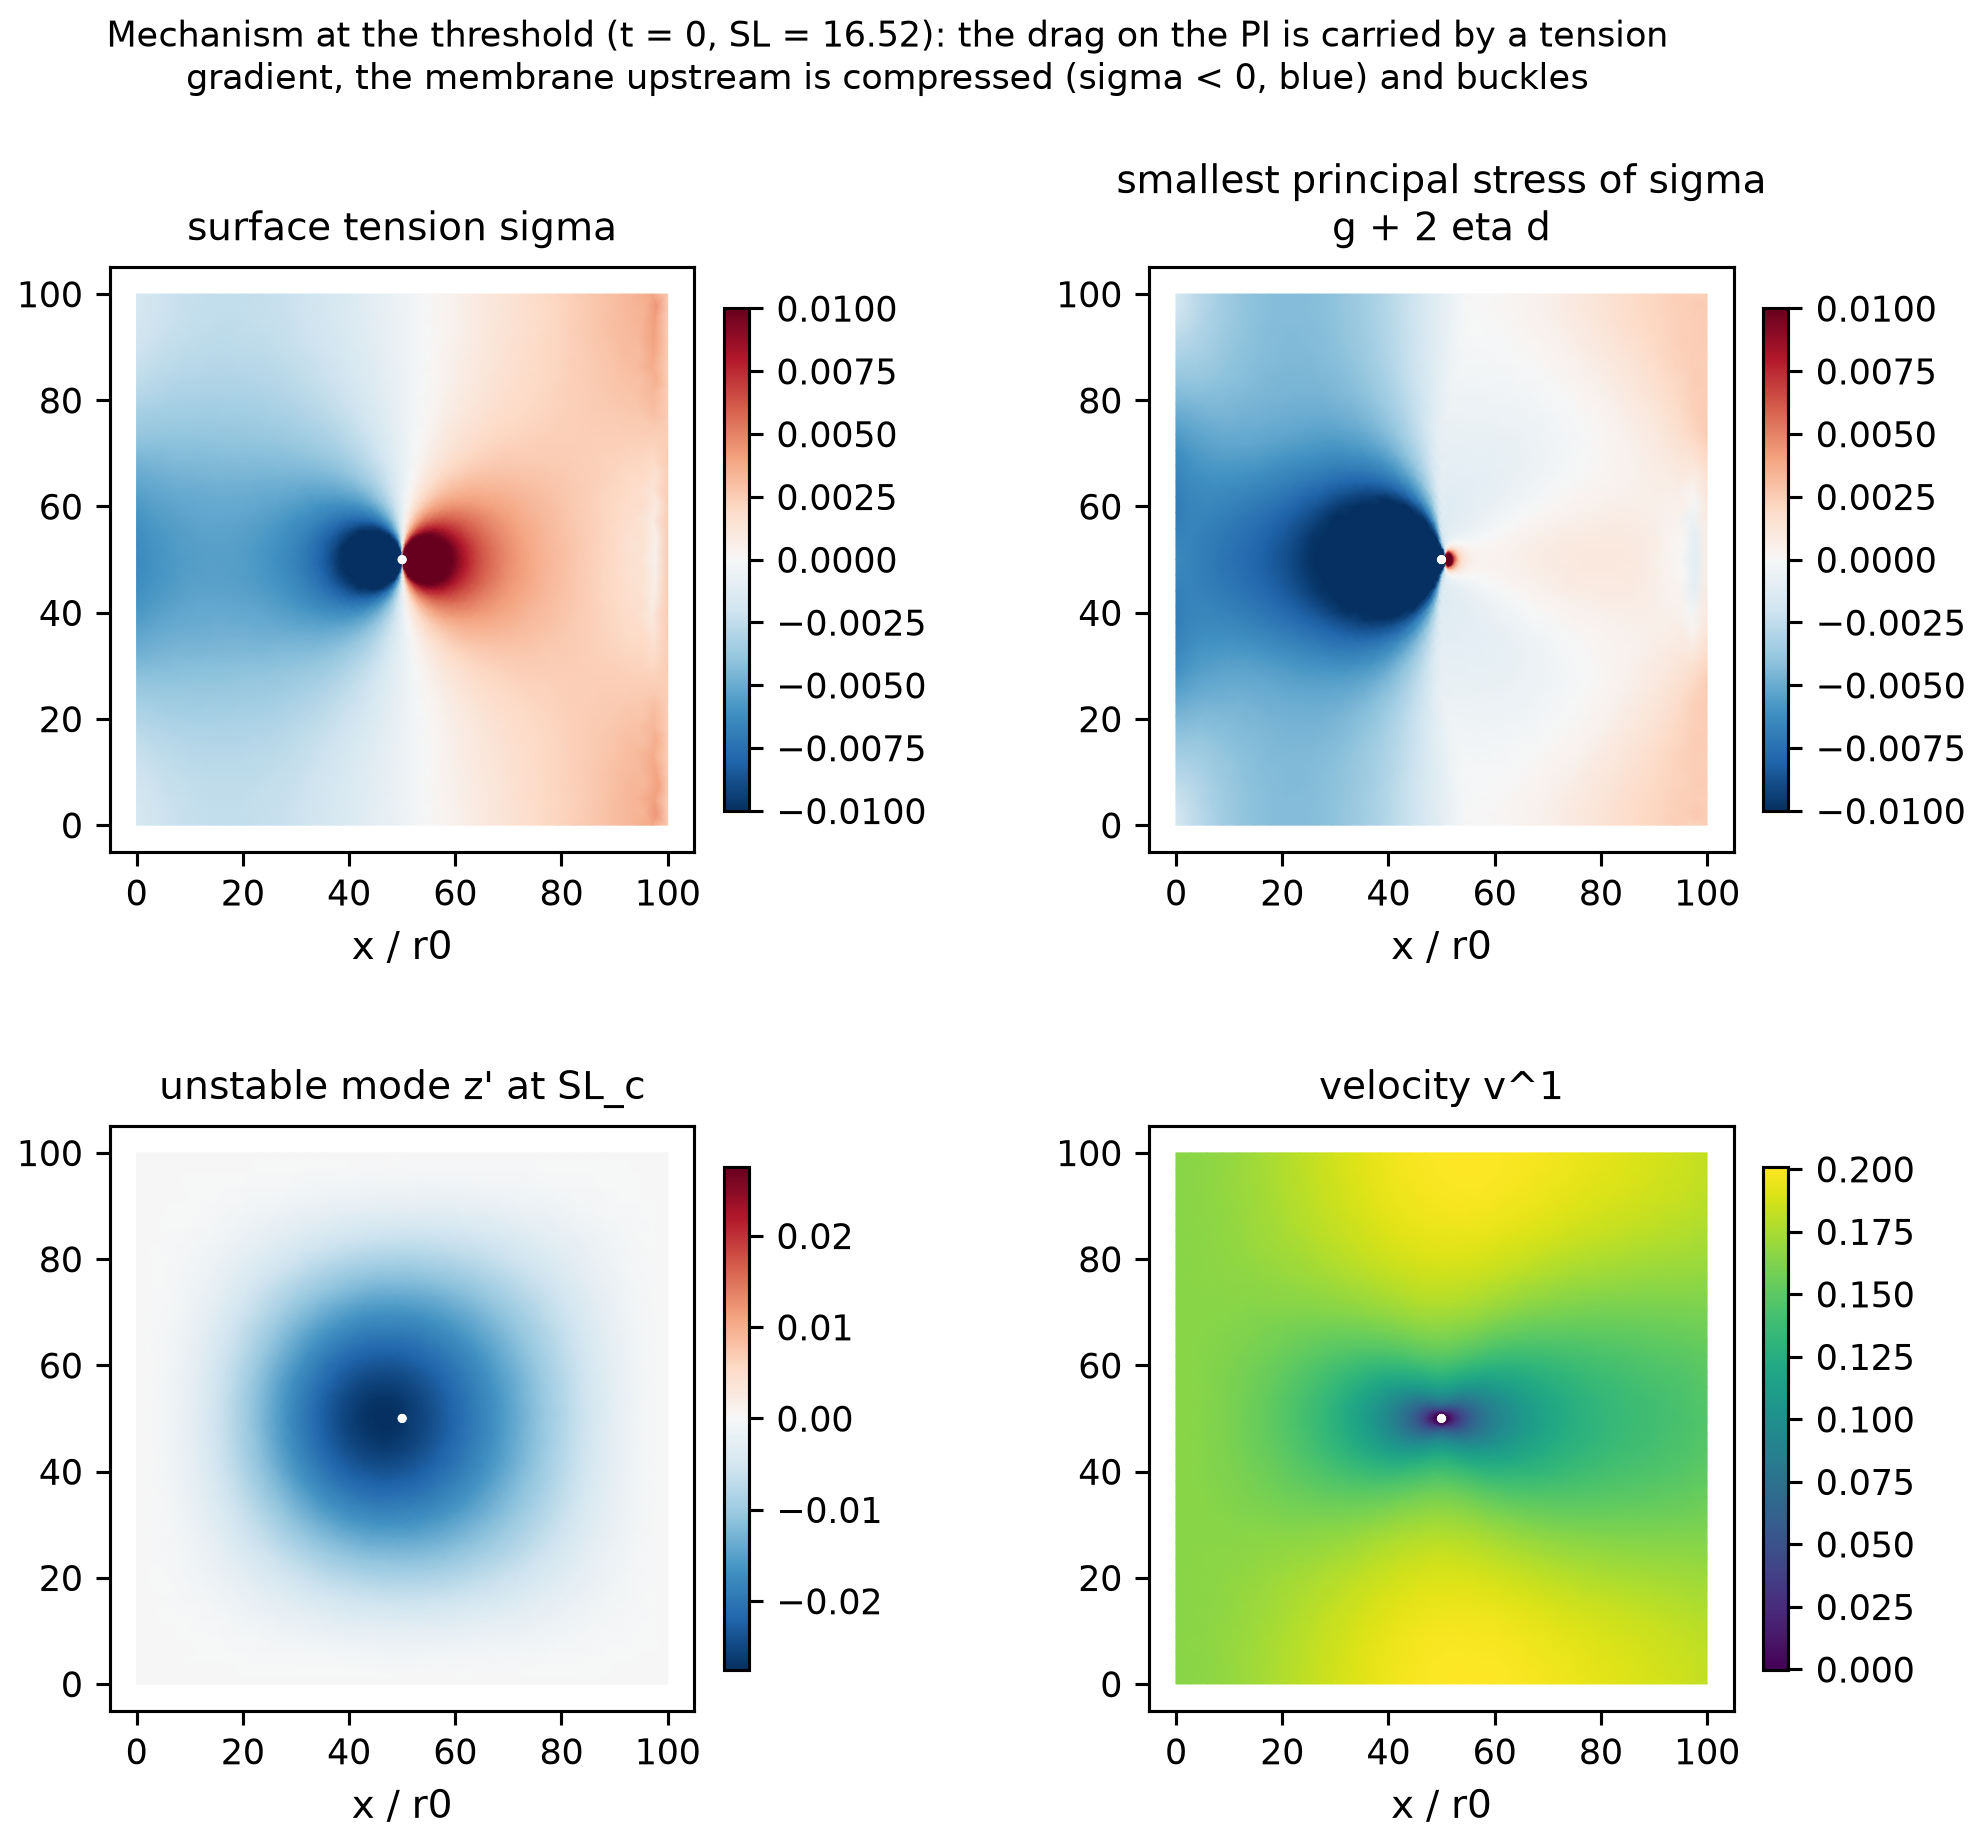
\includegraphics[width=\linewidth,height=140mm,keepaspectratio]{figures/layout/membrane_flow_pre_mechanism.png}%
}
\expandafter\def\csname reportlayout@figures/membrane_flow_pre_imperfect_shapes.png\endcsname{%
  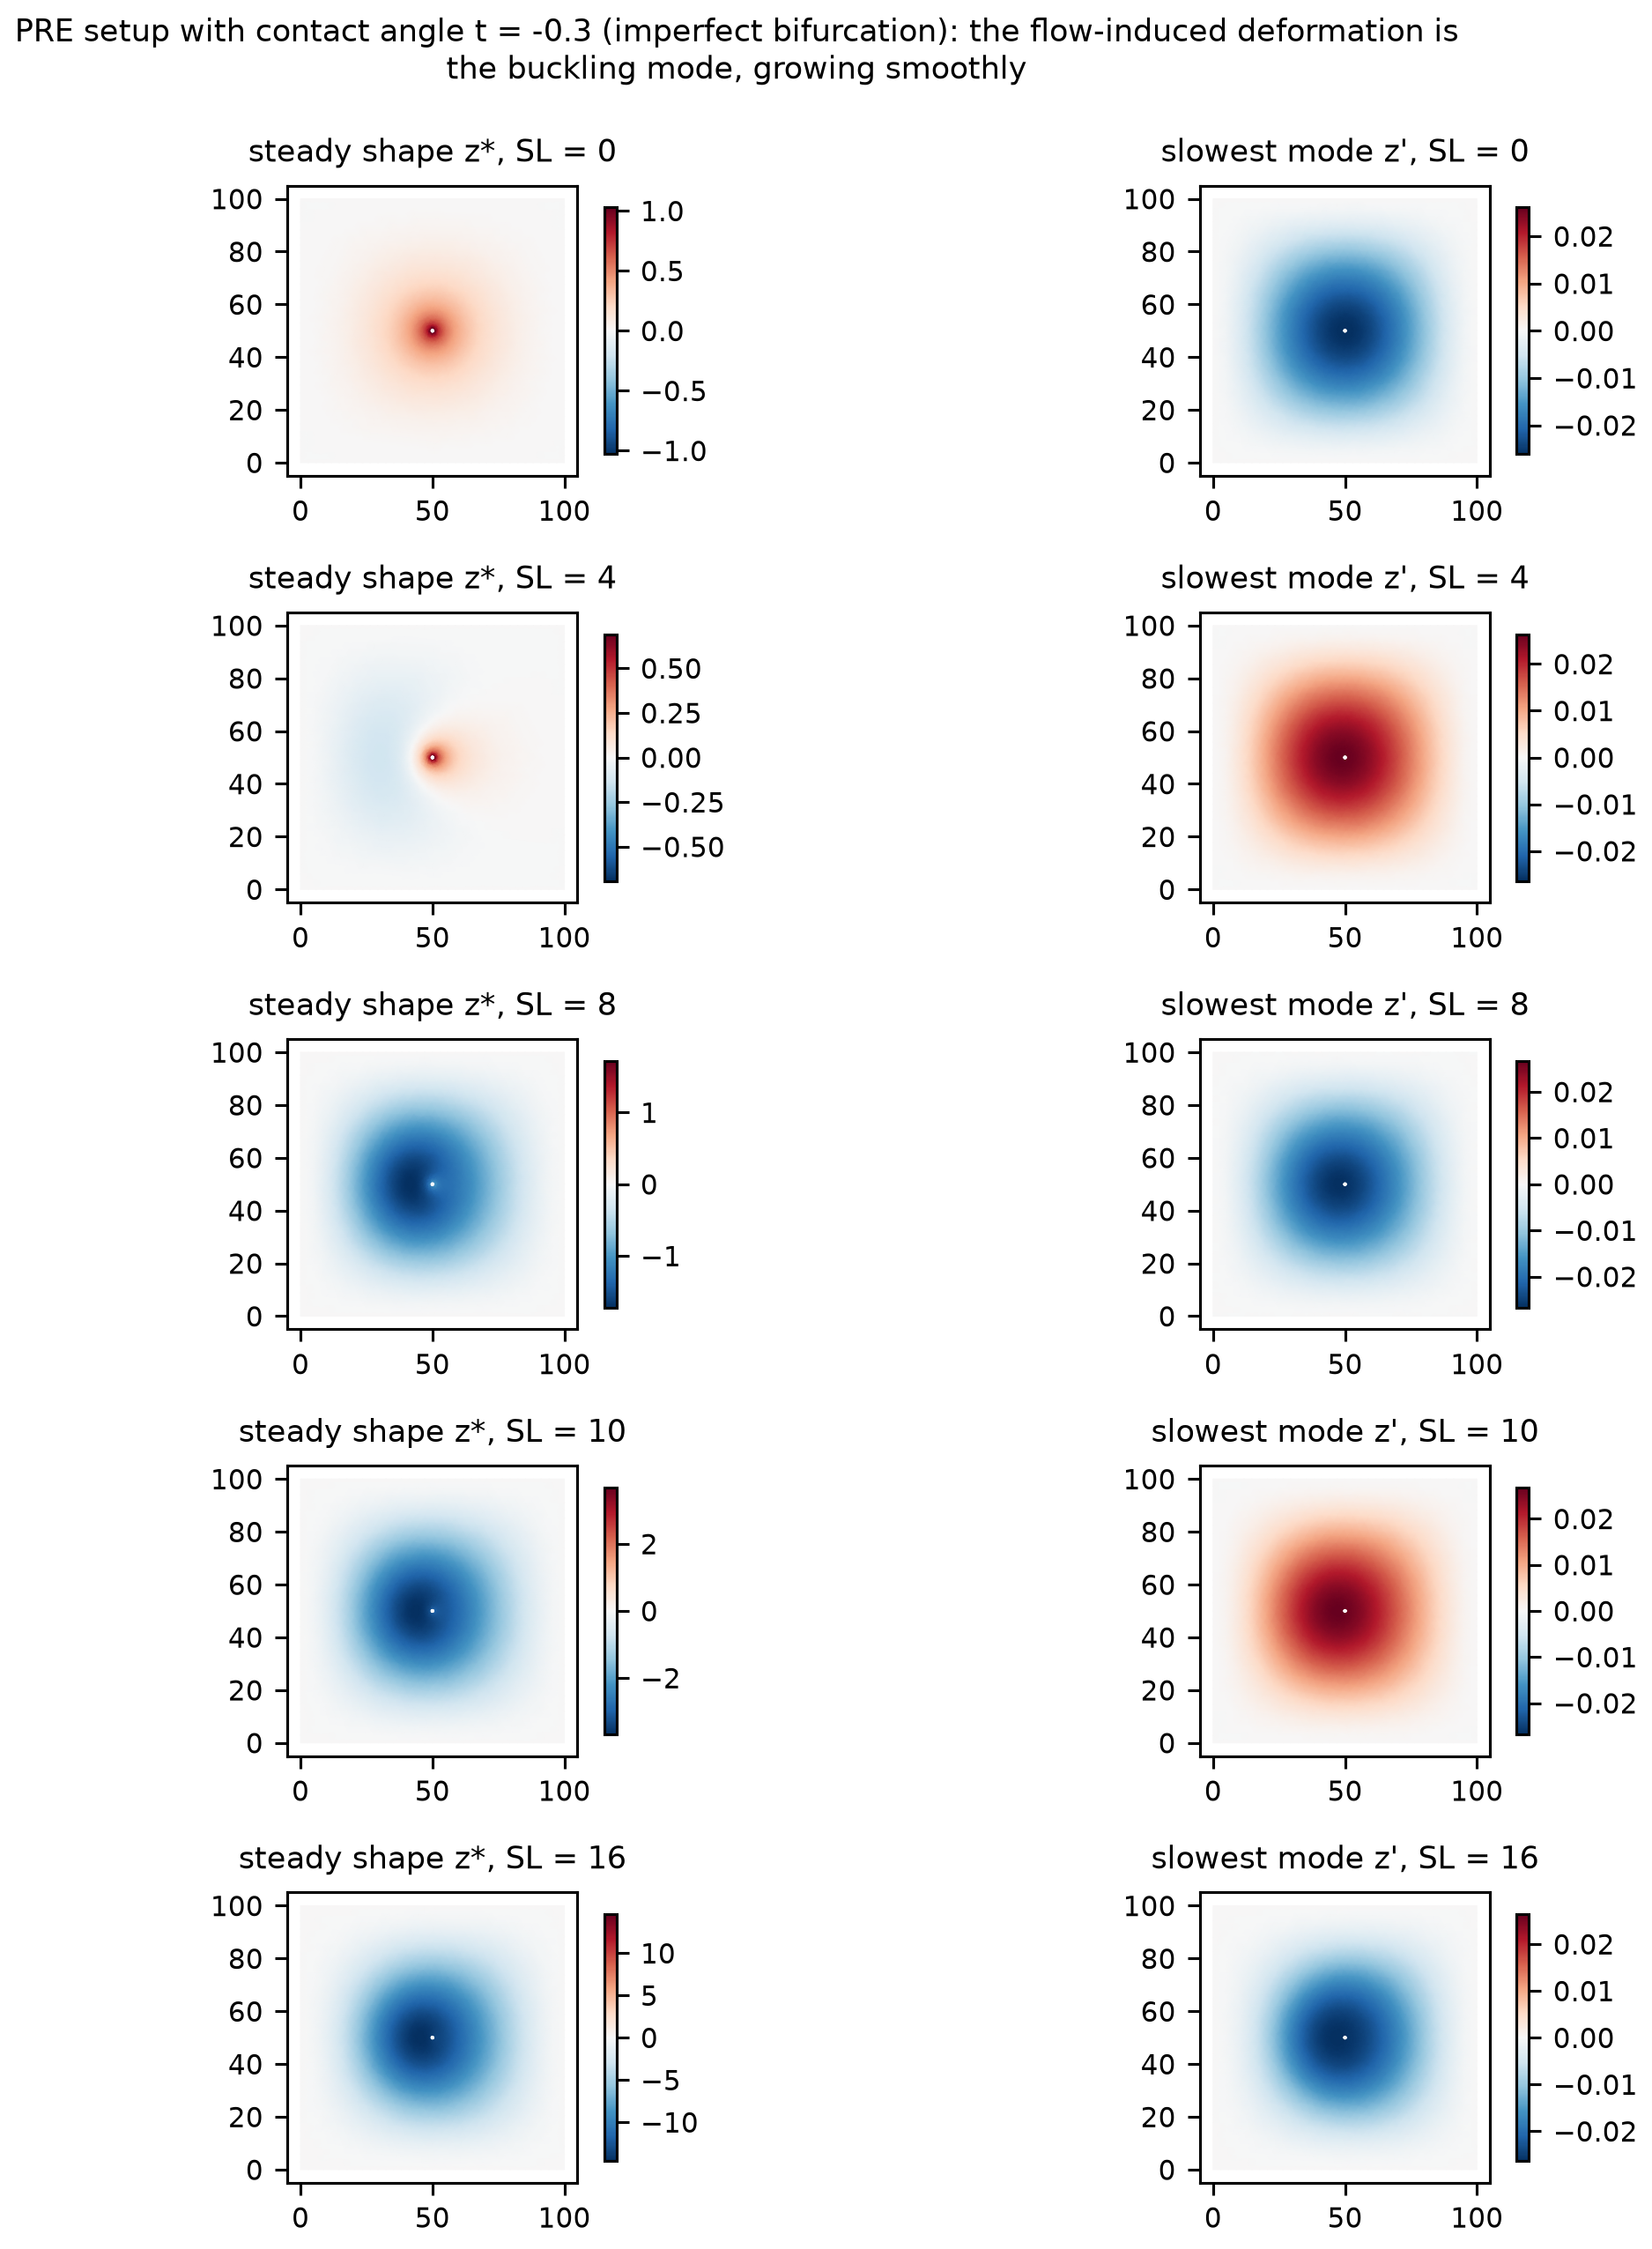
\includegraphics[width=\linewidth,height=220mm,keepaspectratio]{figures/layout/membrane_flow_pre_imperfect_shapes.png}%
}
